\documentclass[11pt]{article}
\usepackage{amsmath,amsbsy,amssymb,verbatim,fullpage,ifthen,graphicx,bm,amsfonts,amsthm}
\usepackage{graphicx}
\usepackage{xcolor}
\usepackage{hyperref}
\usepackage{algorithm}
\usepackage{algpseudocode}
\newcommand{\mfile}[1]  {{\small \verbatiminput{./#1}}} % Jeff Fessler, input matlab file
\newcommand{\tmop}[1]{\ensuremath{\operatorname{#1}}}

\newcommand{\R}{\mathbb{R}}
\newcommand{\C}{\mathbb{C}}
\newcommand{\Z}{\mathbb{Z}}
\newcommand{\A}{\mathcal{A}}
\newcommand{\minimize}{\operatorname*{minimize\ }}
\newcommand{\maximize}{\operatorname*{maximize}}

%\newcommand{\mfile}[1]  {{\small \verbatiminput{./#1}}} 
\newcommand{\mtx}[1]{\mathbf{#1}}
\newcommand{\vct}[1]{\mathbf{#1}}
\def \lg       {\langle}
\def \rg       {\rangle}
\def \mA {\mtx{A}}
\def \mC {\mtx{C}}
\def \mI {\mtx{I}}
\def \mU {\mtx{U}}
\def \mS {\mtx{S}}
\def \mV {\mtx{V}}
\def \mW {\mtx{W}}
\def \mLambda {\mtx{\Lambda}}
\def \mX {\mtx{X}}
\def \mY {\mtx{Y}}
\def \mZ {\mtx{Z}}
\def \zero     {\mathbf{0}}
\def \vzero    {\vct{0}}
\def \vone    {\vct{1}}
\def \vu {\vct{u}}
\def \vv {\vct{v}}
\def \vx {\vct{x}}
\def \vy {\vct{y}}
\def \vz {\vct{z}}
\def \vphi {\vct{\phi}}
\def \vmu {\vct{\mu}}
\def \R {\mathbb{R}}


\usepackage{xspace}

\makeatletter
\DeclareRobustCommand\onedot{\futurelet\@let@token\@onedot}
\def\@onedot{\ifx\@let@token.\else.\null\fi\xspace}

\def\eg{\emph{e.g}\onedot} \def\Eg{\emph{E.g}\onedot}
\def\ie{\emph{i.e}\onedot} \def\Ie{\emph{I.e}\onedot}
\def\cf{\emph{c.f}\onedot} \def\Cf{\emph{C.f}\onedot}
\def\etc{\emph{etc}\onedot} \def\vs{\emph{vs}\onedot}
\def\wrt{w.r.t\onedot} \def\dof{d.o.f\onedot}
\def\etal{\emph{et al}\onedot} \def\st{\emph{s.t}\onedot}
\pagestyle{plain}

\title{{\bf Homework Set 6, CPSC 6430/4430}}
\author{\Large\underline{LastName, FirstName}}
\date{\textbf{\Large\textcolor{red}{Due 05/03/2024, 11:59PM EST}}}

\begin{document}
\maketitle

\section*{DNN Implementation and Application}
Please refer to Jupyter Notebook.
%We reconsider Linear regression:
%\begin{equation}
%	\min\limits_{\vx}\frac{1}{2}\|\mA\vx-\vy\|^2_2
%\end{equation}
%\begin{enumerate}
%	\item Please randomly generate $\mA\in\R^{10000\times 5000}$, compare the time consumption of closed solution given by $(\mA^T\mA)^{-1}\mA^T\vy$ and gradient descent method $\vx^{k+1}=\vx^k-\lambda\mA^T(\mA\vx-\vy)$ by constant stepsize $\lambda=1/\|\mA\|_F^2$ assuming 1000 iterations, which one is faster?
%	\item Please randomly generate $\mA\in\R^{100\times 50}$, compare the time consumption of closed solution given by $(\mA^T\mA)^{-1}\mA^T\vy$ and gradient descent method $\vx^{k+1}=\vx^k-\lambda\mA^T(\mA\vx-\vy)$ by constant stepsize $\lambda=1/\|\mA\|_F^2$ assuming 1000 iterations, which one is faster?
%\end{enumerate}
%(For any matrix $\mZ$, we define $\|\mZ\|_F^2:=\sum\limits_i\sum\limits_j\mZ_{ij}^2$.)
%For PCA, from the perspective of minimizing reconstruction error, please derive the solution to $\minimize \limits_{\bm{\mu},\{\vv_i\},\mU_q} \sum_{i=1}^{N}\|\mX_i-\bm{\mu}-\mU_q \vv_i\|^2_2, \st \ \mU_q^T\mU_q=\mI_q$, where $\mX\in\R^{p\times N}, \bm{\mu}\in\R^p, \mU \in\R^{p\times q}, \vv_i \in \R^q$. 
\newpage
\section*{CNN Implementation and Application}
Please refer to Jupyter Notebook.

%\vspace{.3cm}
%
%\noindent Suppose we wish to use this data set to make a prediction for Y when $X_1=X_2=X_3=0$ using $K$-nearest neighbors ($K$-NN).
%\begin{enumerate}
%	\item Compute the Euclidean distance between each observation and the test point $X_1=X_2=X_3=0$.
%	\item What is our prediction with $K=1$ and why? 
%	\item What is our prediction with $K=3$ and why? Please determine the probability assigning to each class (Red or Green) by using uniform weight or distance weight (where each neighbor's weight is determined by $w_i=\frac{exp\{-d_i^2\}}{\sum_{j=1}^{K}exp\{-d_j^2\}}$ and $d_i$ denotes the Euclidean distance of testing data to $i$-th nearest neighbor data) respectively.
%	\item Now if we only use the first two features $X_1$ and $X_2$, please scatter plot the six observation points and plot the contour for decision boundary by referring to \href{https://stackoverflow.com/questions/45075638/graph-k-nn-decision-boundaries-in-matplotlib}{here}.
%\end{enumerate} 



%For Ridge Regression:
%\begin{equation}
%	\min\limits_{\vx}\|\mA\vx-\vy\|^2_2+\gamma\|\vx\|^2_2,
%\end{equation}
%\begin{enumerate}
%	\item What is the derivative with respect to $\vx$?
%	\item What is the closed solution of ridge regression?
%	\item Assume $\mA\in\R^{100\times50}$, and stepsize $\lambda=0.5/(\gamma+\sigma_1(\mA\mA^T))$, where $\sigma_1(\mZ)$ denotes the largest singular value of $\mZ$. Please change $\lambda$ from $\{0.01, 0.1,1,10,100\}$ and plot the objective changes with update via gradient descent method (100 iterations), what do you find?
%\end{enumerate}

\newpage
\section*{Understanding RNN}
\begin{figure}[h!]
	\centering
	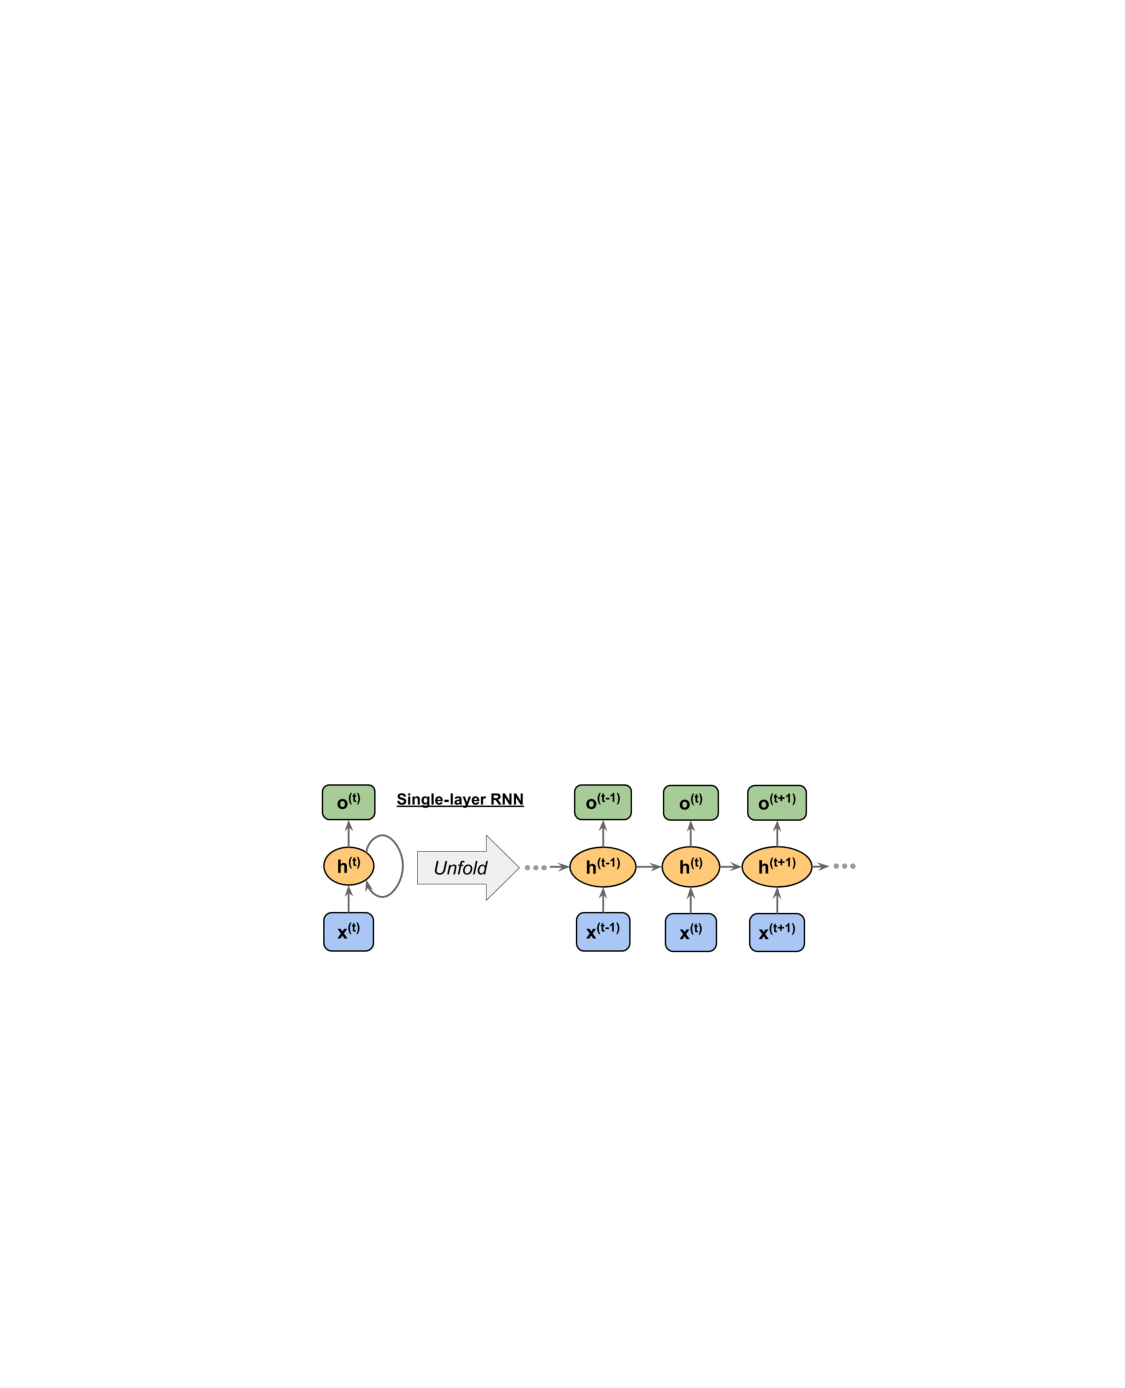
\includegraphics[width=0.9\linewidth]{RNN}
	\caption{Assume $x^{t-1}=[1, 2, 3, 4, 5], x^{t}=[0, 2, 4, 6, 8], x^{t+1}=[0, 1, 2, 3, 5]$.}
	\label{fig:rnn}
\end{figure}
\noindent Assume there is no bias term and $W_{xh}=\begin{bmatrix}
	0 & 1 & 2 & 3 &4 \\ 
	5 &  6& 7 &  8& 9
\end{bmatrix}, W_{hh}=\begin{bmatrix}
2 & 3  \\ 
3 &  7
\end{bmatrix}$. Please determine $h^{t-1},h^{t},h^{t+1}$ where there is no activation function in each step or output.
\newpage
 \section*{Backpropogation}
 Consider the MLP structure as below and the layer $h$ to $z$ is connected with Sigmoid function ($z_i=\frac{1}{1+exp(-h_i)}$) while both $x$ to $h$ and $z$ to $y$ are fully connected layers. The initial weight for $x_i$ and $h_j$ is $i*j$ while $z_k$ and $y_l$ is $(k+1)*(l+1)$. Assume the groundtruth of $y_1, y_2$ is $5,10$ and the loss function is defined by \textit{Mean Squared Error (MSE)}. Given the input $x_1,x_2,x_3$ being $1, 2, 4$ and assume we are using gradient descent method to update the parameters with $stepsize=0.01$ and there is no bias term.
\begin{figure}[h!]
	\centering
	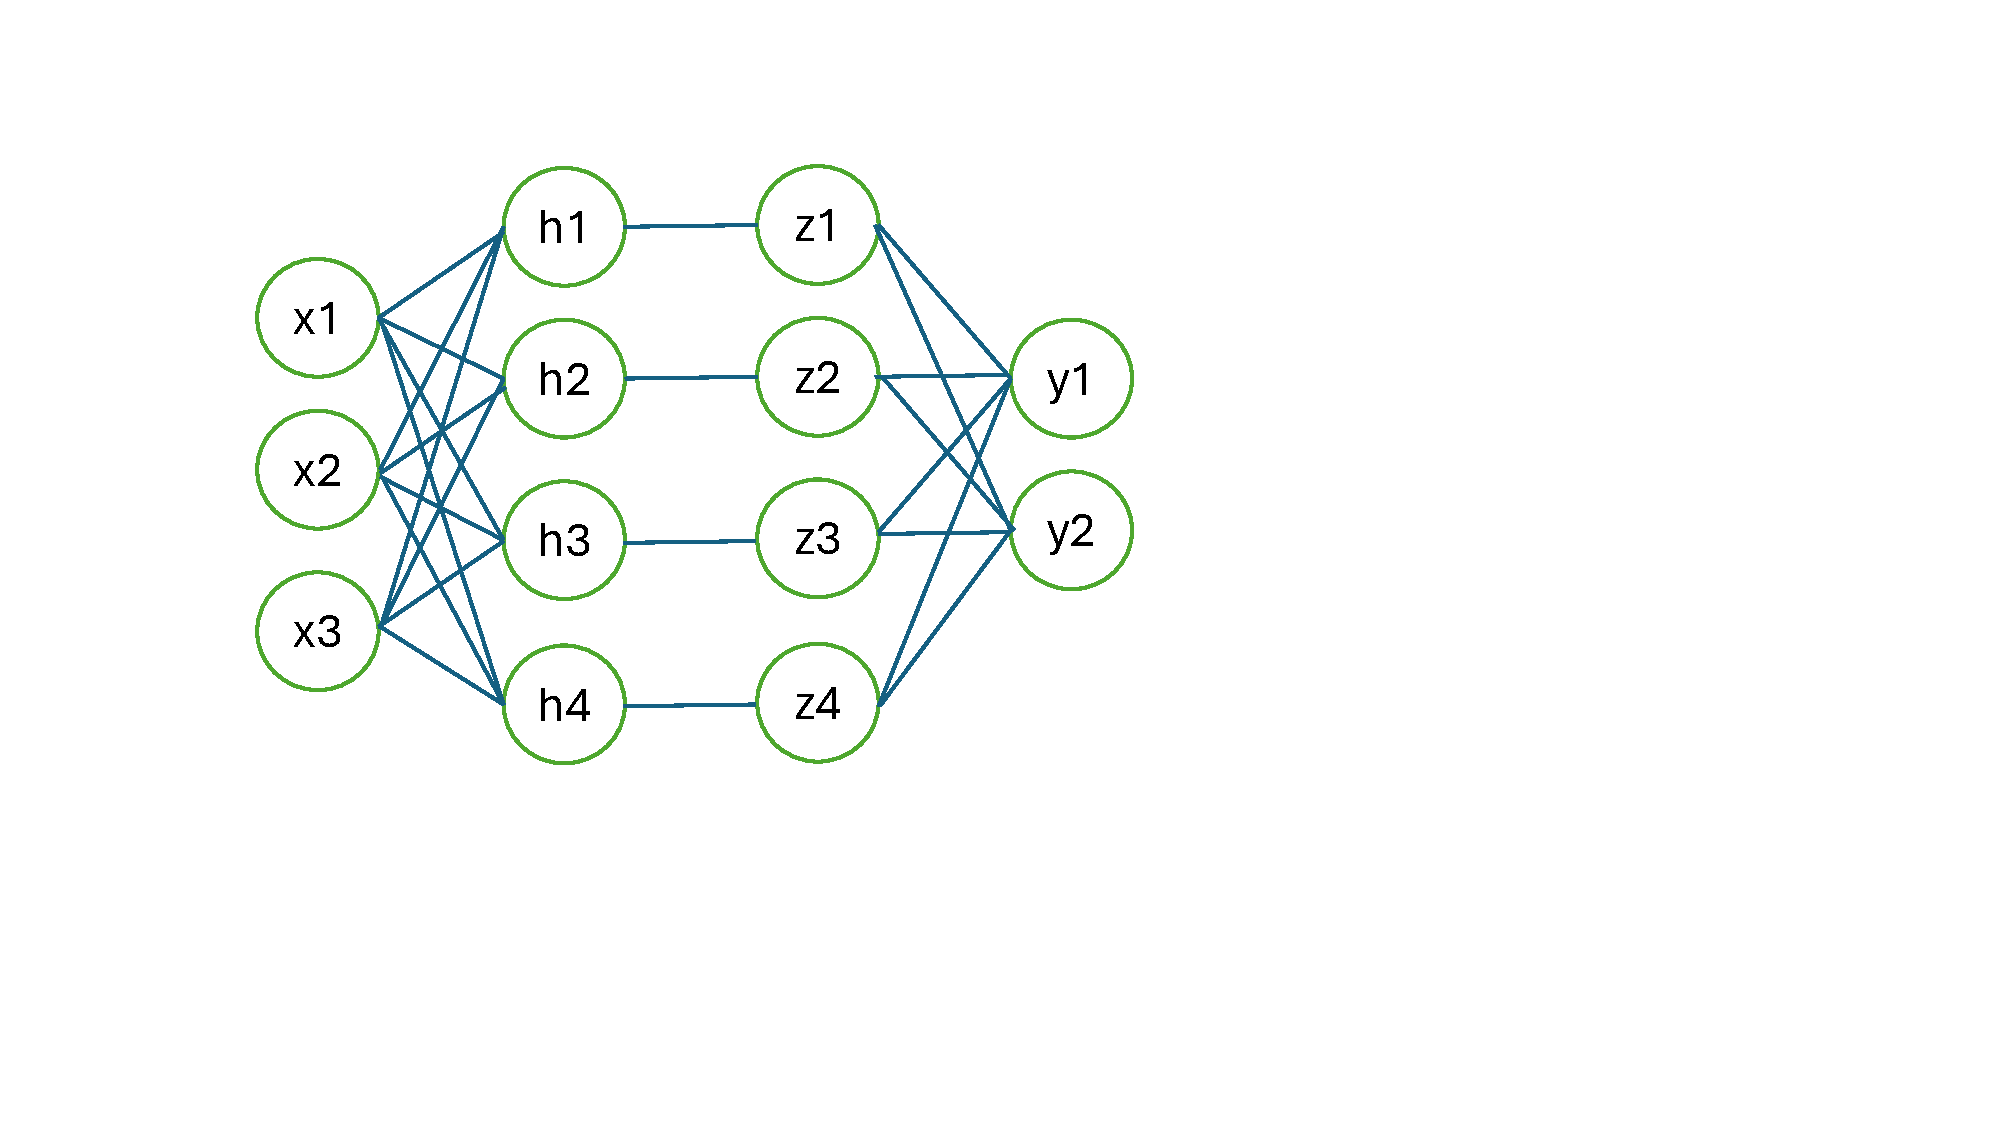
\includegraphics[width=0.6\linewidth]{backprop}
	\caption{}
	\label{fig:backprop}
\end{figure}
\begin{enumerate}
	\item What are the predicted $y_1, y_2$?
	\item How many parameters do we have to learn for this network?
	\item What is the weight to connect $x_1$ with $h_1$  and the weight to connect $z_2$ with $y_1$ after the first update, respectively?
\end{enumerate}
%\end{itemize}
\end{document}
